\chapter*{Popis a rozbor problému }

\par Často řešenou úlohou v oblasti počítačové grafiky a digitální kartografie bývá určování vzájemného vztahu polohy daného bodu a uzavřené oblasti (Bayer 2008). Řešení tohoto úkolu, známého jako \emph{Point-in-Polygon Problem} (PIPP), poskytuje informaci o tom, zda se bod nachází uvnitř, vně nebo na hranici souvislého uzavřeného útvaru (polygonu). Možnosti řešení se pro konvexní a nekonvexní útvary liší zejména v náročnosti algoritmů potřebných pro zohlednění specifických případů polohy vrcholů jednotlivých polygonů (Rourke 2005). Bayer (2023) rozlišuje 2 základní techniky řešení PIPP:

\begin{itemize}
  \item převedení problému na vztah bodu a mnohoúhelníku; 
  \item planární dělení roviny.
\end{itemize}

\par V prvním případě jde o opakované určování polohy bodu vzhledem k mnohoúhelníku; tato technika je snadno implementovatelná, avšak pomalejší. V druhém případě je rovina rozdělena na množinu pásů či lichoběžníků, čímž vzniká \emph{trapezoidální mapa} (Rourke 2005). Rozdělení rovin vede k rychlejšímu nalezení řešení, implementace však bývá obtížnější.
\par Zjištění vzájemné polohy bodu a konvexního útvaru je možné provést jednoduchými algoritmy, například testováním polohy bodu vůči každé hraně útvaru (tzv. \textbf{\emph{Half-plane test}}, složitost \emph{O}(\emph{n})). Nacházejí uplatnění především v triangulačních algoritmech. Mnoho takových algoritmů však nelze použít samo o sobě pro nekonvexní útvary, které se často vyskytují právě v oblasti geoinformatiky a kartografie.
\par Existují dva základní algoritmy vhodné pro nekonvexní útvary schopny detekovat vzájemnou polohu bodu a uzavřené oblasti: \textbf{\emph{Winding Number Algorithm}} a \textbf{\emph{Ray Algorithm}}. Oba tyto algoritmy mají časovou složitost \emph{O}(\emph{n}), přičemž jeden z nich je výrazně rychlejší (Rourke 2005). Těmto algoritmům bude níže věnována samostatná pozornost.

\bigbreak

\section*{Winding Number Algorithm}
\par Winding Number algoritmus je prvním z řešení, kterým lze analyzovat polohu bodu pro nekonvexní mnohoúhelníky. V české literatuře se může označovat jako metoda \emph{ovíjení}. Algoritmus je založen na sčítání/odečítání úhlů, který svírá bod s jednotlivými segmenty polygonu. Za předpokladu, že součet úhlů je \emph{2$\pi$}, pak se bod nachází uvnitř polygonu. Segmentem je uvažována přímka tvořená dvěma po sobě následujícími body v polygonu.
\par Zjednodušeně řečeno, bude-li se pozorovatel dívat z bodu do každého vrcholu v polygonu a bude postupně sčítat úhly, o které se otáčí, součet výsledného úhlu bude 360° (Bayer 2008, Žára 2004).

%\newpage

\par {\large\textbf{Podstata algoritmu} }
\par Mějme uzavřenou oblast \emph{O} v $\mathbb{R}^2$, jejíž hrany tvoří množinou bodů \emph{P} = {$\{P_1, ..., P_n, P_1$\} a bod {\emph{q}}}. Výsledná hodnota algoritmu Winding Number je součet všech uhlů, které opíše průvodič v polygonu. \newline Platí vztah:

\begin{equation}\Omega = \sum_{i=1}^{n} \omega_i.\end{equation}

\par Aby bylo možné spočítat celkový úhel pro daný polygon, je nejprve nutné analyzovat polohu bodu \emph{q} vůči každé přímce, která je definovaná dvěma po sobě následujícími vrcholy $p_i$ a $p_{i+1}$ jež tvoří segment v polygonu. Vzájemná poloha bodu a dané přímky  se vyšetří pomocí Half-plane testu, kde mohou nastat 3 situace (Bayer 2023):

\begin{itemize}
  \item bod q leží vpravo od přímky,
  \item bod q leží vlevo od přímky,
  \item bod q leží na přímce.
\end{itemize}

\par Jako testovací kritérium se použije vztah pro výpočet determinantu matice, která se skládá z vektorů $\vec{p} = (p_x,p_y)$ a $\vec{s} = (s_x,s_y)$:

\begin{equation}\begin{aligned}\vec{p} = p_{i+1} - p_i, \\
 \vec{s} = q - p_i.\end{aligned}\end{equation}

\par Vztah pro výpočet determinantu:
\begin{equation}det = (p_x*s_y)-(s_x*p_y).\end{equation}

\par Pokud
\begin{equation} det\begin{cases} < 0, & \text{bod\emph{ q}\ leží vpravo od přímky} \\ > 0,& \text{bod }q\text{ leží vlevo od přímky} \\ = 0 , & \text{bod }q\text{ leží na přímce} \end{cases}\end{equation}

\par Následně je potřeba procházet jednotlivé hrany v polygonu a sčítat, či odečítat všechny úhly $\omega_i + \omega_{i+1} + ... + \omega_n$ ve směru hodinových ručiečk (nebo v opačném směru) v závislosti na výsledku determinantu. Pro výpočet úhlu $\omega$ je nutné spočíst vektory $\vec{u} = (u_x,u_y)$ a $\vec{v} = (v_x,v_y)$ spočtené jako (viz obrázek 1): 

\begin{equation}\begin{aligned}\vec{u} = p_i - q, \\
                                \vec{v} = p_{i+1} - q .
 \end{aligned}\end{equation}

\begin{figure}[h]
    \centering
        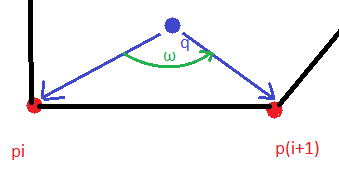
\includegraphics[width=7cm]{uhel} % also works with logo.pdf
    \caption{Úhel vektorů $\vec{u}$ a $\vec{v}$}
\end{figure}

\newpage

\par Velikost úhlu se pak spočítá podle vztahu:
\begin{equation}\cos(\omega) = \frac{\vec{u}\cdot\vec{v}}{||\vec{u}||\cdot||\vec{v}||}\end{equation}

\par Pro následující kroky je nutné pracovat s absolutní hodnotou úhlu $\omega$, jelikož se bude v dalším kroku rozhodovat o jeho přičtení, nebo odečtení.
\begin{equation}|\omega| = \arccos\left(\frac{\vec{u}\cdot\vec{v}}{||\vec{u}||\cdot||\vec{v}||}\right)\end{equation}

\par Bude-li
\begin{equation} det\begin{cases} < 0, & \text{{ pak }$-=\omega$} \\ > 0,& \text{{ pak }$+=\omega$} \end{cases}\end{equation}

\par Následně se všechny úhly sečtou podle vztahu (1) a pokud:
\begin{equation} \Omega\begin{cases} = 2\pi, & \text{\emph{q}}\ \in O, \\ < 2\pi,& \text{\emph{q}} \ \notin O. \\\end{cases}\end{equation}

\par {\large\textbf{Speciální případy algoritmu} }
\par Takto výše popsaný algoritmus bude schopný detekovat bod uvnitř polygonu a mimo něj. Následující část bude věnována případu, kdy se bude analyzovaný bod \emph{q} nacházet na hraně polygonu. Vztah (4) se již částečně o tomto případu zmiňuje. Bod bude ležet na hraně právě tehdy, když
\begin{equation}det = 0.\end{equation}

\par Pro následnou implementaci však pouze tato podmínka nestačí, a proto se dále dá detekovat bod na hraně právě tehdy, když
\begin{equation}\omega = \pi.\end{equation}

\par Výše uvedené dva vztahy ovšem nezohledňují situaci, kdy se bod bude nacházet v jednom z vrcholů množiny \emph{P}. Pro ošetření této možnosti se využije podmínky:
\begin{equation}\text{if\emph{ q}} = p_i\end{equation}
pak se bod nachází ve vrcholu - tedy na hraně polygonu.

\vfill
\par {\large\textbf{Pseudokód} }
\par Na závěr této sekce jsou výše zmíněné kroky shrnuty v pseudokódu, který je implementován v metodě \emph{windingNumberAlgorithm} v souboru \emph{algorithms.py}.
\vfill

\begin{algorithm}[h]
\caption{ Winding Number}\label{alg:cap}
\begin{algorithmic}
\Require $q: bod, pol: polygon$
\Ensure $-1 ,0 ,1$
\State $n \gets {\text{\emph{délka polygonu}}}$
\State $eps \gets {\text{\emph{prahová hodnota}}}$ \Comment{velmi malá kladná hodnota blízká 0}
\State $totalAngle \gets 0$ \Comment{inicializace velikosti úhlu}
\For{všechny vrcholy v polygonu}
    \If{bod je vrchol} 
    \State {\text{\textbf{vrať} hodnotu -1}}\Comment{bod leží na hraně}
    \EndIf

    \State {\text{Spočti vektor \emph{p}:} pi+1 - i}
    \State {\text{Spočti vektor \emph{s}:} q - pi}
    \State {\text{Spočti determinant z vektorů \emph{p} a \emph{s}}}
    \State {\text{Spočti vektor \emph{u}:} pi - q}
    \State {\text{Spočti vektor \emph{v}:} pi+1 - q}
    \State {\text{Spočti úhel $\omega$ z vektorů \emph{u} a \emph{v}}}

    \If{determinant je větší než 0} 
        \State $totalAngle \gets +{\text{$\omega$}}$
    \ElsIf{determinant je menší než 0}
        \State $totalAngle \gets -{\text{$\omega$}}$
    \EndIf
    \If{determinant je 0 a zároveň je úhel (\emph{u} a \emph{v}) - $\pi$ menší než eps} 
        \State {\text{\textbf{vrať} hodnotu -1}} \Comment{bod leží na hraně}
    \EndIf
\EndFor
\If{absolutní hodnota( z (abs. hodnoty totalAngle)) - 2$\pi$ je menší než eps}
    \State {\text{\textbf{vrať} hodnotu 1}} \Comment{bod leží uvnitř polygonu}
\Else{} 
    \State {\text{\textbf{vrať} hodnotu 0}} \Comment{bod leží vně polygonu}
\EndIf
\end{algorithmic}
\end{algorithm}

\newpage

\section*{Ray Crossing Algorithm}
\par Další možné řešení PIPP pro nekonvexní útvary představuje \emph{Ray Crossing Algorithm}, který bývá také označován jako \emph{Ray Algorithm}, \emph{Ray Casting Algorithm} nebo \emph{Even-Odd Rule Algorithm}, v češtině i jako \emph{paprskový algoritmus} (Bayer 2008). Tento algoritmus zjišťuje vzájemný vztah polohy bodu a útvaru na základě počtu průsečníků, které tvoří polopřímka vedena z daného bodu s hranami tohoto útvaru. V případě, že je tento počet lichý, uvažovaný bod se nachází uvnitř polygonu, je –li tento počet sudý nebo rovný nule, uvažovaný bod se nachází vně polygonu. V případě, že je s uvažovaným bodem totožný právě jeden průsečík, tento bod se nachází na hraně polygonu (obrázek 2).

\begin{figure}[h]
\centering
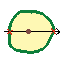
\includegraphics[width=8cm]{raycrossing} % also works with logo.pdf
    \caption{Detekce polohy bodů vzhledem k polygonu za použití Ray Crossing algoritmu (převzato z Rourke 2005, s. 240)}
\end{figure}

\par Tento algoritmus je možné dále modifikovat tak, abychom jeho implementaci zjednodušili a zabránili vzniku problematických situací.

\bigbreak

\par {\large\textbf{Podstata algoritmu} }
\par Mějme uzavřenou oblast \emph{O} v $\mathbb{R}^2$, jejíž hrany tvoří množinou bodů \emph{P} = {$\{P_1, ..., P_n, P_1$\} a bod {\emph{q}}}. Uvažujme vodorovnou testovací přímku \emph{r} procházející bodem \emph{q} takovou, že 
\begin{equation} r(q): y=y_q.\end{equation}

\par Počet průsečíku \emph{k} přímky \emph{r} s oblastí \emph{O} pak určuje polohu bodu \emph{q} vůči \emph{O} tak, že
\begin{equation} k\%2=\begin{cases} 1, & \text{\emph{q}}\ \in O, \\ 0 , & \text{\emph{q}} \ \notin O. \\\end{cases}\end{equation}

\par Tato varianta algoritmu však neřeší případy, když \emph{r}(\emph{q}) prochází vrcholem $P_i$ nebo hranou a neumí detekovat stav, když \emph{q} leží na hraně $\delta$. Pro vylepšení je možné provést modifikaci algoritmu s redukcí ke \emph{q} a rozdělením \emph{r} na dvě polopřímky $r_1$ a $r_2$ s opačnou orientací: nechť je $r_1$ levostranná a $r_2$ pravostranná polopřímka. Udržujme si počet levostranných a pravostranných průsečíků $k_l$ a $k_r$. Zavedeme–li si lokální souřadnicový systém s počátkem v bodě \emph{q} a osami \emph{x'}, \emph{y'} a polopřímky  $r_1(q)$ a $r_2(q)$ ztotožníme s osou \emph{x'} tak, že je možné je popsat rovnicí (Bayer 2023)
\begin{equation} y' = 0,\end{equation}

\par můžeme provést redukci bodů $p_i = [x_i, y_i]$ ke $q$:
\begin{equation}\begin{aligned}x'_i = x_i - x_q, \\
                               y'_i = y_i - y_q.
 \end{aligned}\end{equation}
 
\par Pokud průsečík $M = [x'_m, y'_m = 0]$ segmentu (hrany) oblasti \emph{O} a osy \emph{x'} (jedné z polopřímek \emph{x'}, \emph{y'}) existuje, můžeme ho určit ze vztahu
\begin{equation}x'_m = \frac{x'_{i+1}y'_i - x'_iy'_{i+1}}{y'_{i+1}-y'_i}.\end{equation}

\par Podmínky existence průsečíku $M$ s jednou z polopřímek $r_1(q)$, $r_2(q)$ udávají vztahy:
\begin{itemize}
    \item pro levou polorovinu: 
        \begin{equation} t_l = y_{i+1} < y_q \neq y_i < y_q,\end{equation}
    \item pro pravou polorovinu:
        \begin{equation} t_r = y_{i+1} > y_q \neq y_i > y_q,\end{equation}
\end{itemize}

\par kde $t_l$, $t_r$ nabývají hodnoty \verb|True| nebo \verb|False|. Průsečík $M$ se pak vypočte pro každou polopřímku zvlášť:
\begin{itemize}
    \item pokud $t_l$ = \verb|True| $\land$ $x'_m$ < 0, inkrementujeme $k_l$,
    \item pokud $t_r$ = \verb|True| $\land$ $x'_m$ > 0, inkrementujeme $k_r$.
\end{itemize}

\par Jinak řečeno: Průsečíky pro levou a pravou část budeme započítávat v případě, leží –li počáteční a koncový bod protnutého segmentu v jiné polorovině (vrchní nebo spodní). Pak
\begin{equation} q =\begin{cases} \in \delta $O$, & \text{$k_l\%2 \neq k_r\%2$,} \\ 
    \in \emph{O}, & \text{$k_r\%2 = 1$,} \\ 
    \notin \emph{O}, & \text{jinak.} 
\end{cases}\end{equation}

\par {\large\textbf{Speciální případy algoritmu} }
\par Při řešení PIPP pomocí \emph{Ray Algorithm} může docházet k případům, které je nutno dodatečně ošetřit.
\par Pokud je zvolený bod $q$ totožný s jedním z bodů $p_i$, pak je možné prohlásit, že $q \in \delta O$.
\par Pokud přímka $r(q)$ prochází vrcholem oblasti $O$, může nastat detekce dvou průsečíku (koncový bod jednoho segmentu a počáteční bod druhého segmentu). Situaci je možné ošetřit započtením tohoto vrcholu jako průsečíku jenom jednou (Bayer 2008, Rourke 2005).

\par Pokud platí, že 
\begin{equation}y_{i+1} - y_i = 0,\end{equation}
\par pak body tvoří $p_{i+1}$ a $p_i$ horizontální hranu a výpočet průsečíku ze vztahu (17) nebude možný. Ve vlastní implementaci algoritmu se v tom případě pokračuje následující iterací.
\par Může nastat situace, když se bod $p_i$ chybně zařadí do vrchní nebo spodní poloroviny oblasti $O$, pokud tento bod leží velmi blízko testovací přímky $r(q)$. Je proto vhodné zavést prahovou hodnotu $\varepsilon$, která tento případ ošetří:
\begin{equation}|y_i - y_q| \leq \varepsilon.\end{equation}

\par {\large\textbf{Pseudokód} }
\par Vlastní implementace \emph{Ray Crossing Algorithm} je níže shrnuta v pseudokódu. Nachází se v metodě \emph{rayCrossingAlgorithm} v souboru \emph{algorithms.py}.

\bigbreak

\begin{algorithm}[h]
\caption{ Ray Crossing}\label{alg:cap}
\begin{algorithmic}
\Require $q: bod, pol: polygon$
\Ensure $-1 ,1 ,0$
\State $kr \gets {\text{\emph{počet pravostranných průsečníků}}}$
\State $kl \gets {\text{\emph{počet levostranných průsečníků}}}$ 
\State $n \gets {\text{\emph{délka polygonu}}}$
\For{všechny vrcholy v polygonu}
    \State Spočti $x_i$, $y_i$
    \If{bod je vrchol} \Comment{bod leží na hraně}
    \State {\text{\textbf{vrať} hodnotu -1}}
    \EndIf

    \State Spočti $x_{i+1}, y_{i+1}$
    \If{ ($y_{i+1} - y_i) == 0$} \Comment{horizontální segment}
    \State {\text{\textbf{pokračuj novou iterací}}}
    \EndIf
    \State Spočti průsečník $x'_m$
    \If{ $y_{i+1} < y_q \neq y_i < y_q$} \Comment{spodní segment}
        \If{ $x'_m < 0$} \Comment{průsečník v levé polrovině}
         \State Inkrementuj $k_l$
        \EndIf
    \EndIf
    \If{ $y_{i+1} > y_q \neq y_i > y_q$} \Comment{vrchní segment}
        \If{ $x'_m > 0$} \Comment{průsečník v pravé polrovině}
         \State Inkrementuj $k_r$
        \EndIf
    \EndIf
\EndFor

\If{$k_l\%2 \neq k_r\%2$}
    \State {\text{\textbf{vrať} hodnotu -1}}  \Comment{bod leží na hraně}
\ElsIf{$k_r\%2 = 1$}
    \State {\text{\textbf{vrať} hodnotu 1}}  \Comment{bod leží uvnitř polygonu}
\Else{}
    \State {\text{\textbf{vrať} hodnotu 0}}  \Comment{bod leží vně polygonu}
\EndIf
\end{algorithmic}
\end{algorithm}